\documentclass[aps,prb,preprint,groupaddress,floatfix]{revtex4}

\usepackage{graphicx}
\usepackage{dcolumn}
\usepackage{bm}
\usepackage{amsmath}
\usepackage{multirow}
\usepackage{xcolor}
\usepackage{simpler-wick}
\usepackage{cases}

\newcommand{\tbh}[3]{\multicolumn{#1}{#2}{\textbf{#3}}}
\newcommand{\tbhc}[1]{\multicolumn{1}{c}{\textbf{#1}}}
\newcommand{\tbhl}[1]{\multicolumn{1}{l}{\textbf{#1}}}
\newcommand{\tbhr}[1]{\multicolumn{1}{r}{\textbf{#1}}}
\newcommand{\tbr}[1]{\multicolumn{1}{r}{#1}}
\newcommand{\tbc}[1]{\multicolumn{1}{c}{#1}}
\newcommand{\fnm}[1]{\footnotemark[#1]}
\newcolumntype{f}[1]{D{.}{.}{#1}}

\renewcommand{\deg}[0]{$^{\circ}$}

\begin{document}


\title{Supplementary Information: Real-time coupled-cluster approach for the cumulant Green's function}
\date{\today}

\author{F. D. Vila}
\author{J. J. Rehr}
\author{J. J. Kas}
\affiliation{Department of Physics, University of Washington, Seattle, WA 98195}
\author{K. Kowalski}
\affiliation{William R. Wiley Environmental Molecular Sciences Laboratory, Battelle, Pacific Northwest National Laboratory, K8-91, P. O. Box 999, Richland, Washington 99352}
\author{B. Peng}
\affiliation{Physical Sciences Division, Pacific Northwest National Laboratory, Richland, WA 99354}

\begin{abstract} 
This Supplementary Information presents results that are too detailed for the main manuscript, including more detailed discussion of the theory derivations in the main manuscript, computational details, results for other basis sets, and more results that are too technical for the main manuscript.
\end{abstract}

\date{\today}

\maketitle

\section{Theory}

\subsection{Retarded Green's function in spin-orbital basis}


The real-space, real-time retarded Green's function is defined as
\begin{equation}
\label{eq:gfrtrs}
\begin{split}
G(x,x') =& ~ G(rt,r't') = \\
&-i \Theta(t-t')\left<0\left| \left\{\psi(rt), \psi^\dagger(r't') \right\} \right| 0 \right>
\end{split}
\end{equation}
where $\left| 0 \right>$ is the ground state of the system, $\psi^\dagger(r't')$
and $\psi(rt)$ are, respectively, the creation and annhilation field operators
at $r't'$ and $rt$, and $\left\{,\right\}$ indicates the anticonmutation
operator. By introducing a basis set of single-particle spin-orbitals
$\{\phi_p(r)\}$, we can express any two-positions, two-times operator $M$ as:
\begin{equation}
\label{eqn:mel1}
M(rt,r't') = \sum_{pq} \phi^{*}_{p}(r) M_{pq}(t,t') \phi_{q}(r')
\end{equation}
where the matrix elements are defined as:
\begin{equation}
\label{eqn:mel2}
M_{pq}(t,t') = \int dr dr' \phi^{*}_{p}(r) M(rt,r't') \phi_{q}(r').
\end{equation}
Inserting these definitions into Eq. (\ref{eq:gfrtrs}) we obtain the Green's function matrix expressed in the spin-orbital basis $\{\phi_p(r)\}$:
\begin{equation}
\label{eqn:gpq}
G_{pq}(t,t') =
-i \Theta(t-t')
\left<0\left| \left\{a_p(t), a_q^\dagger(t') \right\} \right| 0 \right>,
\end{equation}
where the creation and annhilation operators $a_p^\dagger(t)$ and $a_q(t')$ are
associated with the spin-orbitals $\phi_p$ and $\phi_q$ respectively.

\subsection{From the real-space time-domain Dyson equation to the cumulant ansatz in a spin-orbital basis}

The real-space, time-domain form of the Dyson equation
\begin{equation}
\begin{split}
G(x,x') =&~ G^0(x,x') + \\
&\int dx_1 dx_2 G^0(x,x_1) \Sigma(x_1,x_2) G(x_2,x')
\end{split}
\end{equation}
can also be cast in matrix form (after including time translation invariance):
\begin{equation}
\label{eqn:dyson}
\hat{G}(t) = \hat{G}^0(t) + \int dt_1 dt_2 \hat{G}^0(t-t_1)
\hat{\Sigma}(t_1-t_2) \hat{G}(t_2).
\end{equation}
Expanding the matrix form of the cumulant ansatz
\begin{equation}
\label{eqn:cummat}
\hat{G}(t) = \hat{G}^0(t)e^{\hat{C}(t)},
\end{equation}
and Eq. (\ref{eqn:dyson}) to first order
\begin{eqnarray}
\hat{G}(t) &=& \hat{G}^0(t) + \hat{G}^0(t)\hat{C}(t) + ... \\
\hat{G}(t) &=& \hat{G}^0(t) + \int dt_1 dt_2 \hat{G}^0(t-t_1)
\hat{\Sigma}(t_1-t_2) \hat{G}^0(t_2) + ...
\end{eqnarray}
and equating the second terms in the right hand sides we get:
\begin{equation}
\hat{G}^0(t)\hat{C}(t) = \int dt_1 dt_2 \hat{G}^0(t-t_1)
\hat{\Sigma}(t_1-t_2) \hat{G}^0(t_2)
\end{equation}
For a typical matrix element we obtain
\begin{equation}
\sum_r G^0_{pr}(t) C_{rq}(t) = \sum_{rs} \int dt_1 dt_2 G^0_{pr}(t-t_1)
\Sigma_{rs}(t_1-t_2) G^0_{sq}(t_2),
\end{equation}

Shifting the $\omega$ integration variable and using the Fourier transform of
the cumulant we have:
\begin{equation}
C_{pq}(\omega) = i G^0_{pp}(\omega+\epsilon_p)
\Sigma_{pq}(\omega+\epsilon_p) G^0_{qq}(\omega+\epsilon_p).
\end{equation}
Finally, introducing the frequency domain form of
$G^0_{pp}=(\omega-\epsilon_p+i\delta)^{-1}$:
\begin{equation}
\label{eqn:cumfreq}
C_{pq}(\omega) = \frac{i \Sigma_{pq}(\omega+\epsilon_p)}
{(\omega+i\delta)(\omega+\epsilon_p-\epsilon_q+i\delta)}.
\end{equation}
If we approximate $\Sigma_{pq}(\omega) \simeq \Sigma_{pp}(\omega) \delta_{pq}$,
then
\begin{equation}
\label{eqn:cum_diag}
C_{pp}(\omega) = \frac{i \Sigma_{pp}(\omega+\epsilon_p)}
{(\omega+i\delta)^2},
\end{equation}
or, in the time domain
\begin{equation}
\label{eqn:cum_diag_t}
C_{pp}(t) = \int \frac{d\omega}{2\pi} \frac{i\Sigma_{pp}(\omega+\epsilon_p)}
{(\omega+i\delta)^2} e^{-i\omega t}.
\end{equation}
We can now return to the time domain, inserting into Eq.\ (\ref{eqn:cummat}) and
taking into account that the matrix exponential is now diagonal:
\begin{equation}
\label{eqn:g_cum_diag}
G_{pp}(t) = i \Theta(t) e^{-i \epsilon_p t + C_{pp}(t)},
\end{equation}
which is the standard form of the diagonal cumulant.

\subsection{Coupled Cluster Green's function in time}
\label{sec:ccg_t}

In this section we derive a compact form for the full Coupled Cluster Green's function that can be used for further derivation of time-domain approximations. Starting with Eq.\ (17)
in Ref. \onlinecite{PhysRevA.94.062512} (from now on referred as ``PK'') we have
\begin{equation}
\label{eq:GPK1}
G^R_{pq} (\omega) = \left< \Phi \left| (1+\Lambda) e^{-T} a^{\dagger}_q
\left( \omega + (H-E_0) -i\delta \right)^{-1}
a_p e^{T} \right| \Phi \right>
\end{equation}
and inserting the $I=e^{-T}e^{T}$ we get
\begin{equation}
\label{eq:GPK2}
G^R_{pq} (\omega) = \left< \Phi \left| (1+\Lambda) \bar{a^{\dagger}_q}
\left( \omega + \bar{H}_N \right)^{-1}
\bar{a}_p \right| \Phi \right>
\end{equation}
where $\bar{O} = e^{-T}Oe^{T}$ is the similarity transformed form of the $O$
operator, $H_N$ is the normal ordered hamiltonian, and using the
Baker-Campbell-Hausdorff (BCH) relation we have that
\begin{equation}
\label{eq:apbar}
\bar{a}_p = a_p + [a_p,T],
\end{equation}
\begin{equation}
\label{eq:aqbar}
\bar{a^{\dagger}_q} = a^{\dagger}_q + [a^{\dagger}_q,T].
\end{equation}
For simplicity, we now make the convergence factor $-i\delta$ implicit in the energy $\omega$.

Following PK, we introduce the $X_p(\omega)$, $Z_q(\omega)$, and $W_q(\omega)$
operators, which are solutions to the following equations:
\begin{equation}
X_{p}(\omega) \left| \Phi \right> = 
\left( \omega + \bar{H}_N \right)^{-1}
\bar{a}_p \left| \Phi \right>,
\end{equation}
\begin{equation}
\left< \Phi \right| Z_{q}(\omega) = 
\left< \Phi \right| (1+\Lambda) \bar{a^{\dagger}_q}
\left( \omega + \bar{H}_N \right)^{-1},
\end{equation}
and
\begin{equation}
\left< \Phi \right| (1+\Lambda) W_{q}(\omega) = 
\left< \Phi \right| (1+\Lambda) \bar{a^{\dagger}_q}
\left( \omega + \bar{H}_N \right)^{-1}
\end{equation}
These operators have the following expansions in the $N-1$ Fock space:
\begin{equation}
\label{eq:Xomega}
\begin{split}
X_{p}(\omega) =& \sum_i x^i(\omega)_p a_i +\\
&\frac{1}{2!}\sum_{ij,a} x^{ij}_a(\omega)_p a^{\dagger}_a a_j a_i + ...
\end{split}
\end{equation}
\begin{equation}
\label{eq:Zomega}
\begin{split}
Z_{q}(\omega) =& \sum_i z_i(\omega)_q a^{\dagger}_i +\\
&\frac{1}{2!}\sum_{ij,a} z_{ij}^a(\omega)_p a^{\dagger}_i a^{\dagger}_j a_a + ...
\end{split}
\end{equation}
and
\begin{equation}
\label{eq:Womega}
\begin{split}
W_{q}(\omega) =& \sum_i w_i(\omega)_q a^{\dagger}_i +\\
&\frac{1}{2!}\sum_{ij,a} w_{ij}^a(\omega)_p a^{\dagger}_i a^{\dagger}_j a_a + ...
\end{split}
\end{equation}

Eqs. (\ref{eq:GPK1})-(\ref{eq:Womega}) are a summary of the formulation in PK. Now, using
\begin{equation}
\mathrm{IFT}\left[\left( \omega + \bar{H}_N -i\delta \right)^{-1} \right] =
i \Theta(-t) e^{i \bar{H}_N t}
\end{equation}
where $\mathrm{IFT}$ is the inverse Fourier transform, we can write
$G^R_{pq} (\omega)$ in the time-domain as:
\begin{equation}
G^R_{pq}(t) = i \left< \Phi \left| (1+\Lambda) \bar{a^{\dagger}_q}
e^{i \bar{H}_N t}
\bar{a}_p \right| \Phi \right>
\end{equation}
where from now on we assume that $t<0$ to remove all the $\Theta(-t)$ functions.
We can also convert the equations defining the $X_p(\omega)$, $Z_q(\omega)$,
and $W_q(\omega)$ operators as:
\begin{equation}
\label{eq:xpt}
X_{p}(t) \left| \Phi \right> = 
i e^{i \bar{H}_N t}
\bar{a}_p \left| \Phi \right>,
\end{equation}
\begin{equation}
\label{eq:zqt}
\left< \Phi \right| Z_{q}(t) = 
i \left< \Phi \right| (1+\Lambda) \bar{a^{\dagger}_q}
e^{i \bar{H}_N t}
\end{equation}
and
\begin{equation}
\label{eq:wqt}
\left< \Phi \right| (1+\Lambda)W_{q}(t) = 
i \left< \Phi \right| (1+\Lambda) \bar{a^{\dagger}_q}
e^{i \bar{H}_N t}
\end{equation}
where the $X_p(t)$, $Z_q(t)$, and $W_q(t)$ are defined simply by the inverse
Fourier transform of their coefficients in their excitation expansions (Eqs. (\ref{eq:Xomega})-(\ref{eq:Womega})).

%---------------------------------------------------------------------------
Based on the properties of the $\bar{H}_N$, i.e., where one assumes that the CC
equations $Q\bar{H}_N|\Phi\rangle = 0$ are satisfied, where $Q$ denotes the
projection operator onto the space spanned by excitations with respect to
$|\Phi\rangle$ Slater determinants, we can prove that, in full analogy with
the frequency representation, the $X_p(t)$ operator can be expressed in terms
of connected diagrams only. To this end we expand $X_p(t)$ in term of powers of
the $\bar{H}_N$ operator
\begin{eqnarray}
X_p(t)|\Phi\rangle &=& ie^{i\bar{H}_Nt} \bar{a_p}|\Phi\rangle \;, \label{step1} \\
&=& i \lbrace \sum_{n=0}^{\infty} \frac{1}{n!} (i)^n t^n (\bar{H}_N)^n \bar{a_p}\rbrace |\Phi\rangle \label{step4} 
\end{eqnarray}

Now we assume that we are dealing with the exact CC theory. This assumption
plays a crucial role in proving the connected character of $X_p(t)$ since all
approximate approaches can be build using connected properties of the exact 
formulation. Using Wick's theorem for the particle-hole formalism to analize a general term in the expansion in Eq. (\ref{step4}):
\begin{equation}
(\bar{H}_N)^n \bar{a_p} |\Phi\rangle,
\label{gterm}
\end{equation}
we can identify several classes of diagrams contributing to $(\bar{H}_N)^n
\bar{a_p} |\Phi\rangle$ (see Figs. (\ref{fig2_conn}) and (\ref{fig3_conn})). It can be easily verified that all disconnected diagrams (typical examples of
these are shown in Fig. (\ref{fig2_conn}a-\ref{fig2_conn}d)) disappear due
to the existence of vertices representing projections of CC equations (i.e., $\bar{H}_N$ matrix elements with all particle-hole creation lines,
that is, all ``legs'', located to the left of the corresponding matrix element or diagrammatic vertex, see Fig. (\ref{fig2_conn}a-\ref{fig2_conn}c)) or due to the existence of the uncontracted particle-hole line (lines) that annihilates the reference function $|\Phi\rangle$ as shown in Fig. (\ref{fig2_conn}d). Consequently, the only diagrams contributing to $X_p(t)$ are connected diagrams
(Fig.(\ref{fig3_conn})) which can be symbolically denoted as 
\begin{equation}
X_p(t)|\Phi\rangle = i
\lbrace e^{i\bar{H}_Nt }\bar{a_p} \rbrace_C |\Phi\rangle\;,
\label{connxp}
\end{equation}
where the subscript ``C'' designates connected part of a given operator expression. 
%
%
\begin{figure}
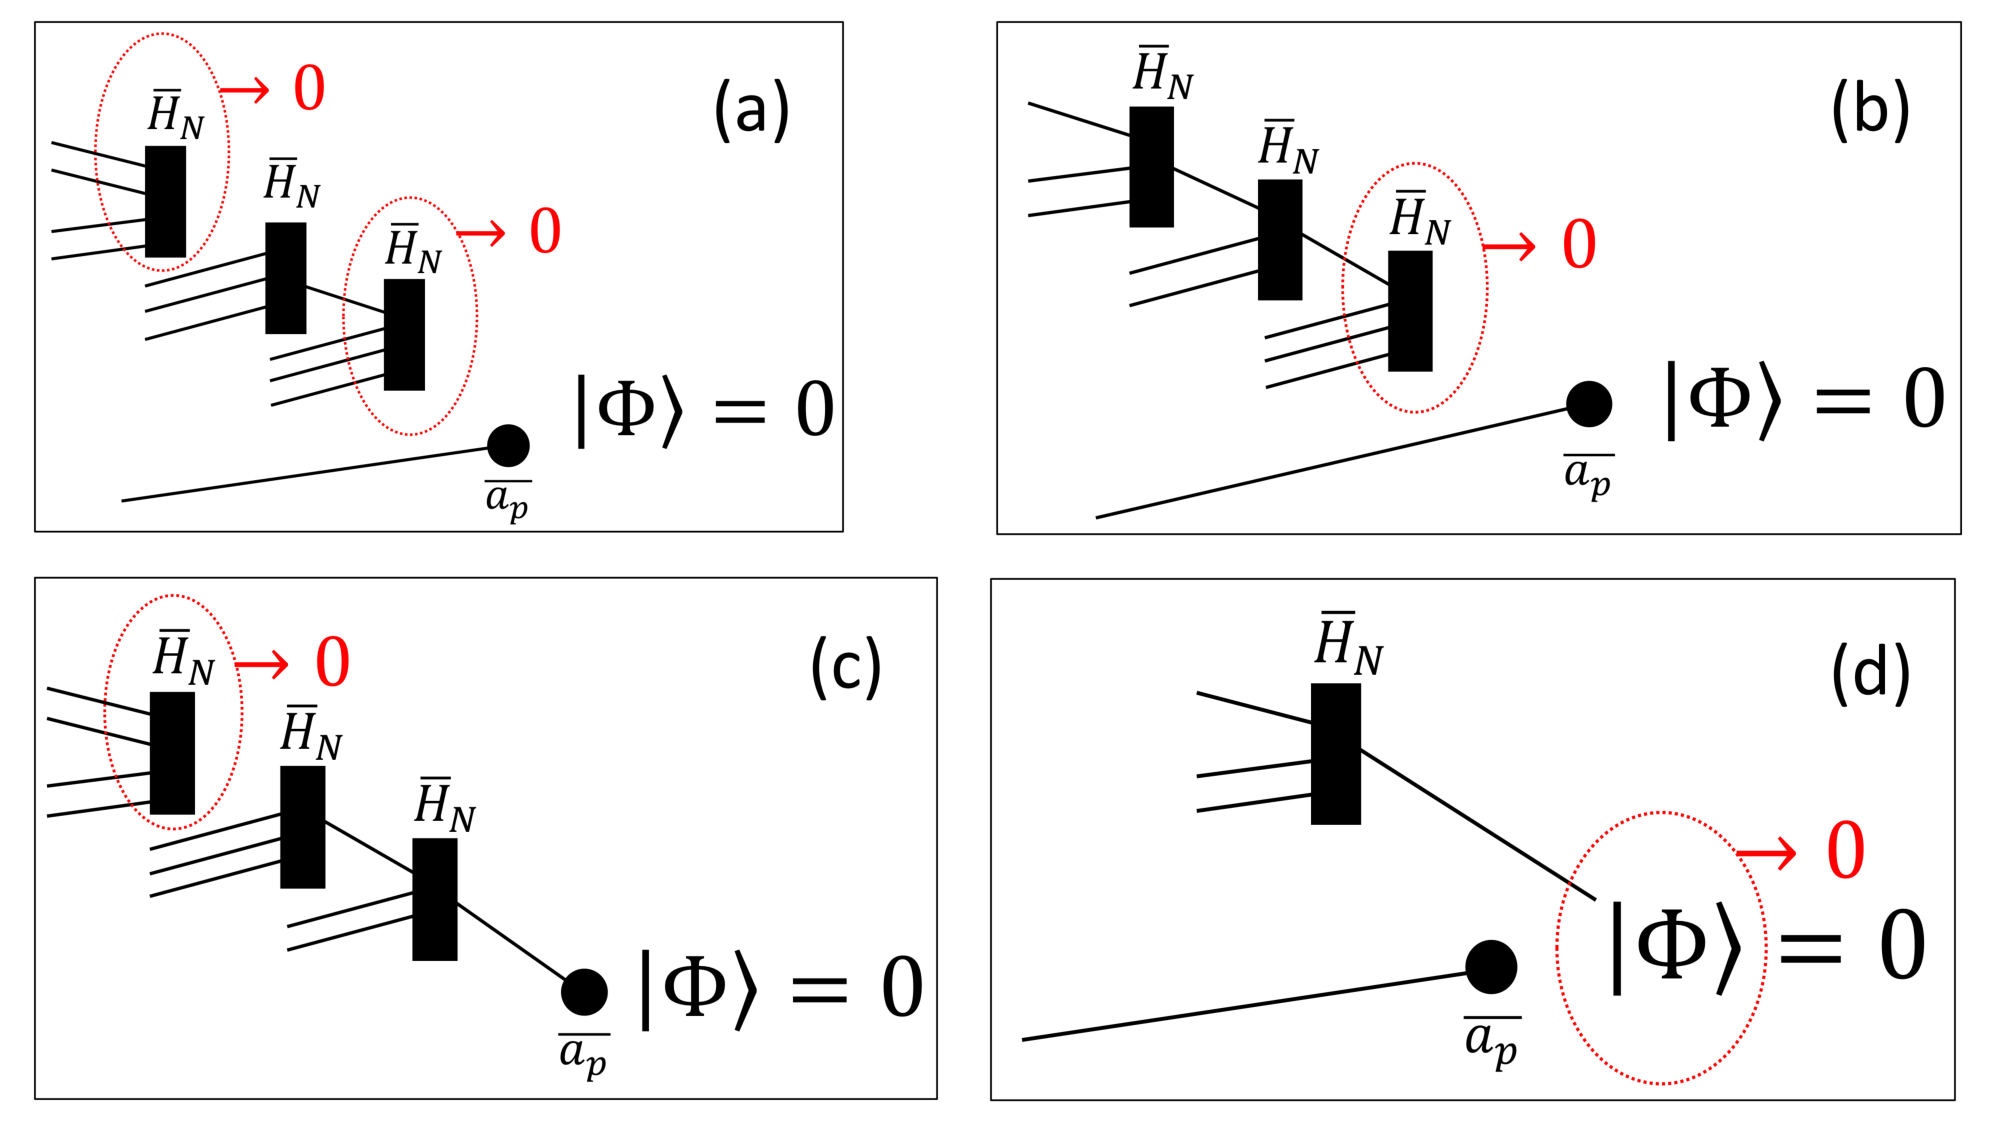
\includegraphics[trim= 0.0in 0.5in 0.0in 0.0in, width=0.65\textwidth]{Fig01-SI.pdf}
\caption{Typical examples of diagrams not contributing to the general term in Eq. (\ref{gterm}).}
\label{fig2_conn}
\end{figure}
%
\begin{figure}
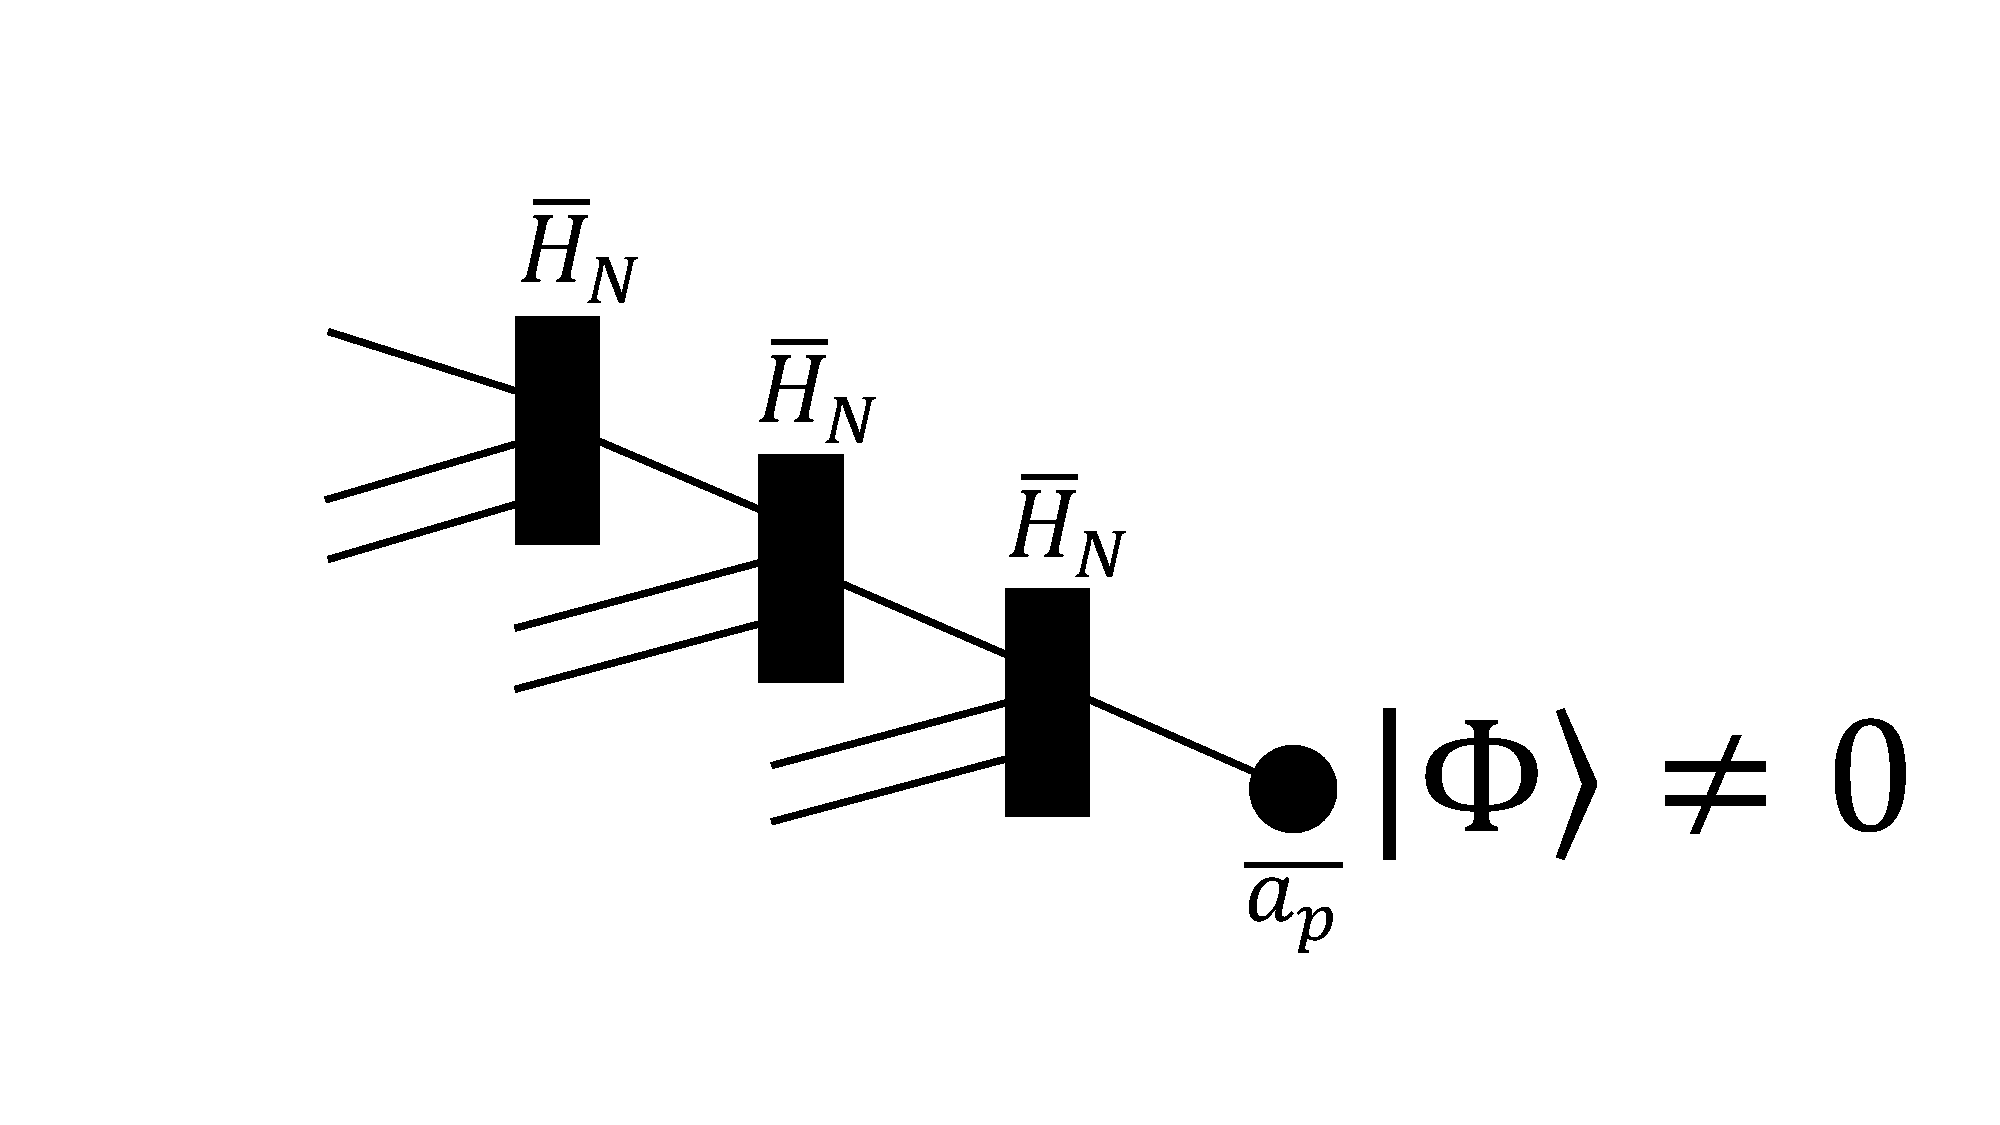
\includegraphics[trim= 0.0in 2.0in 0.0in 1.0in, width=0.45\textwidth]{Fig02-SI.pdf}
\caption{Example of a connected diagram that contributes to the general term in Eq. (\ref{gterm}).}
\label{fig3_conn}
\end{figure}
%
%---------------------------------------------------------------------------


Using the equations above for $X_p(t)$, $Z_q(0^-)$, and $W_q(0^-)$, we can re-write $G^R_{pq}(t)$ as:
\begin{equation}
\label{eq:GZX}
\begin{split}
G^R_{pq}(t)=& \left< \Phi \left| (1+\Lambda)
              \bar{a^{\dagger}_q} X_p(t) \right| \Phi \right> \\
           =& -i \left< \Phi \left|
                Z_q(0^-) X_p(t) \right| \Phi \right> \\
           =& -i \left< \Phi \left| (1+\Lambda)
                W_q(0^-) X_p(t) \right| \Phi \right>
\end{split}
\end{equation}
The first equality is just the time-domain version of Eq. (27) in PK. Note that the $Z_q$ and $W_q$ operators are computed as the limit $ t\rightarrow 0^-$ to avoid any issues with the poorly defined nature of
$\Theta(-t)$ at 0.

We now proceed to expand the second equality in Eq. (\ref{eq:GZX}). We choose to expand this form of $G^R_{pq}(t)$ because it does not include the $\Lambda$ terms (which are implicit in the definition of $Z_{q}(0^-)$) and is thus simpler. Inserting the time dependent definitions of $X_p(t)$ and $Z_q(0^-)$
into $G^R_{pq}(t)$ we have
\begin{multline}
\label{eq:gr_t_sum1}
iG^R_{pq}(t)=
\left< \Phi \right|
\bigl(\sum_i z_i(0^-)_q \{a^{\dagger}_i\} + 
\frac{1}{2!}\sum_{ij,a} z_{ij}^a(0^-)_p \{a^{\dagger}_i a^{\dagger}_j a_a\} + ...\bigr)\\
\bigl(\sum_k x^k(t)_p \{a_k\} +
\frac{1}{2!}\sum_{kl,b} x^{kl}_b(t)_p \{a^{\dagger}_b a_l a_k\} + ...\bigr)
\left| \Phi \right>
\end{multline}
where, to simplify the rest of the calculations, we also introduced the normal
ordered forms of the operators, indicated using Bartlett's style notation
$\{...\}$ rather than the PK one with $N[...]$. Before going any further it is helpful to analyze the general form of a generic matrix element for the different products:
\begin{equation}
\left< \Phi \right|
\{\underbrace{a^{\dagger}_i a^{\dagger}_j ... a_b a_a }_{n~\mathrm{ops}}\}
\{\underbrace{a^{\dagger}_c a^{\dagger}_d ... a_l a_k }_{m~\mathrm{ops}}\}
\left| \Phi \right> =
\sum_\mathrm{FC}
\left< \Phi \right|
\wick{
\{\c3 a^{\dagger}_i \c4 a^{\dagger}_j ... \c1 a_b \c2 a_a
  \c1 a^{\dagger}_c \c2 a^{\dagger}_d ... \c3 a_l \c4 a_k \}
}
\left| \Phi \right>
\end{equation}
where, according to the generalized Wick's theorem (GWT), we compute the Fermi
vacuum expectation value of the product of two normal ordered operator sets by
summing over all possible full contractions (FC). However, for $n \neq m$, the
are no possible full contractions between the two operator sets, thus, the
``cross'' terms in Eq.\ (\ref{eq:gr_t_sum1}) are all zero. For example, we are
only left with terms of the form:
\begin{equation}
\left< \Phi \right|
\{a^{\dagger}_i \} \{a_k \}
\left| \Phi \right> =
\left< \Phi \right|
\wick{
\{\c1 a^{\dagger}_i \c1 a_k \}
}
\left| \Phi \right> = \delta_{ik}
\end{equation}
for 0 excitation order (\textit{i.e.} order 1 in PK),
\begin{multline}
\left< \Phi \right|
\{a^{\dagger}_i a^{\dagger}_j a_a \}
\{a^{\dagger}_b a_l a_k \}
\left| \Phi \right> =
\left< \Phi \right|
\wick{
\{ \c2 a^{\dagger}_i \c3 a^{\dagger}_j \c1 a_a
   \c1 a^{\dagger}_b \c2 a_l \c3 a_k \}
}
\left| \Phi \right>
+
\left< \Phi \right|
\wick{
\{ \c3 a^{\dagger}_i \c2 a^{\dagger}_j \c1 a_a
   \c1 a^{\dagger}_b \c2 a_l \c3 a_k \}
}
\left| \Phi \right> = \\
- \delta_{il}\delta_{jk}\delta_{ab} + \delta_{ik}\delta_{jk}\delta_{ab}
\end{multline}
for 1 excitation order (\textit{i.e.} order 2 in PK), etc. The pattern is fairly
clear: each order produces $h! \times p!$, where $h$ and $p$ are the number of
hole and particle operators in the products. Thus PK order 1 produces one term,
order 2 produces 2, order 3 would produce 12, etc. Thus we can write:
\begin{equation}
iG^R_{pq}(t)=
\sum_i z_i(0^-)_q x^i(t)_p +
\frac{1}{4}\sum_{ij,a} z_{ij}^a(0^-)_p x^{ij}_a(t)_p - 
\frac{1}{4}\sum_{ij,a} z_{ij}^a(0^-)_p x^{ji}_a(t)_p + ...
\end{equation}
This sum can be generalized by recognizing that the $x^{ij}_a(t)_p$ coefficients
are antisymmetric with respect to index swaps, and that $x^{ii}_a(t)_p=0$, thus
\begin{equation}
\begin{split}
iG^R_{pq}(t)=&\\
&\sum_i z_i(0^-)_q x^i(t)_p + \\
+\frac{1}{2}&\sum_{ij,a}   z_{ij}^a(0^-)_p           x^{ij}_a(t)_p + \\ 
+\frac{1}{6}&\sum_{ijk,ab} z_{ijk}^{ab}(0^-)_p x^{ijk}_{ab}(t)_p + ...
\end{split}
\end{equation}

\subsection{Perturbation theory of $G^R_{pq}(t)$}

In this section we demonstrate that the full form of the Coupled Cluster Green's function can be reduced to a cumulant form when approximated as a perturbations series. Although this analysis is valid for any CC level (CCD, CCSD, CCSDT, etc.) with HF orbitals and Moller Plesset MBPT, here for simplicity we limit the CC expansion to doubles ($T=T_2=\frac{1}{4}\sum_{ijab}t_{ij}^{ab} a^{\dagger}_a a^{\dagger}_b a_j a_i$, $\Lambda=\Lambda_2=\frac{1}{4}\sum_{ijab}\lambda_{ij}^{ab} a^{\dagger}_i a^{\dagger}_j a_b a_a$) and expand the $\bar{a}_p$ and $\bar{a^{\dagger}_q}$ operators into their connected forms:
\begin{equation}
\label{eq:gpqrw3}
\begin{split}
G^R_{pq} (\omega) &=\\
&\left< \Phi \left| (1+\Lambda_2)
(a^{\dagger}_q + (a^{\dagger}_q T_2)_C)
X_{p}(\omega) \right| \Phi \right> +\\
&\left< \Phi \left| (1+\Lambda_2)
(a_p + (a_p T_2)_C)
Y_{q}(\omega) \right| \Phi \right>
\end{split}
\end{equation}
where the $X_p$ and $Y_q$ operators are
\begin{equation}
X_{p}(\omega) \left| \Phi \right> = (\omega+\bar{H}_N+i\delta)^{-1}
\bar{a}_p \left| \Phi \right>,
\end{equation}
\begin{equation}
Y_{q}(\omega) \left| \Phi \right> = (\omega-\bar{H}_N+i\delta)^{-1}
\bar{a}^{\dagger}_q \left| \Phi \right>,
\end{equation}
with components
\begin{equation}
X_{p}(\omega) = \sum_i x^i(\omega)_p a_i +
\frac{1}{2!}\sum_{ij,a} x^{ij}_a(\omega)_p a^{\dagger}_a a_j a_i = X_{1,p}(\omega)+X_{2,p}(\omega),
\end{equation}
\begin{equation}
Y_{q}(\omega) = \sum_a y_a(\omega)_q a^{\dagger}_a +
\frac{1}{2!}\sum_{i,ab} y^i_{ab}(\omega)_q a^{\dagger}_a a^{\dagger}_b a_i = Y_{1,q}(\omega)+Y_{2,q}(\omega).
\end{equation}
We proceed in the frequency domain because this simplifies the perturbation analysis. Each term in Eq.\ (\ref{eq:gpqrw3}) generates six possible terms, but, analyzing their corresponding diagrams we can see that there are only three non-zero terms when $p,q \in occ$:
\begin{equation}
\label{eq:gpqrw4}
G^R_{pq} (\omega) =
\left< \Phi \left| a^{\dagger}_q X_{1,p}(\omega) \right| \Phi \right> +
\left< \Phi \left| \Lambda_2 (a^{\dagger}_q T_2)_C
X_{1,p}(\omega) \right| \Phi \right> +
\left< \Phi \left| \Lambda_2 a_p Y_{2,q}(\omega) \right| \Phi \right>.
\end{equation}
After computing each term we get:
\begin{equation}
\label{eq:gpqrw5}
G^R_{pq} (\omega) =
x^q(\omega)_p -\frac{1}{2} \sum_{ijab} \lambda^{ab}_{ij} t^{qj}_{ab}
x^i(\omega)_p
-\frac{1}{2} \sum_{iab} \lambda^{ab}_{pi} y^{i}_{ab}(\omega)_q.
\end{equation}
This is the form of the Green's function which can be used to approximate $G^R_{pq}$ using perturbation theory. For this purpose we
write each of the coefficients in Eq.\ (\ref{eq:gpqrw5}) up to second order in a perturbation parameter $\lambda$, e.g. $t_{pq}^{rs} = t_{pq}^{(0)rs} + \lambda t_{pq}^{(1)rs} + \lambda^2 t_{pq}^{(2)rs}$, etc. By
keeping only terms up to second order we get:
\begin{equation}
\label{eq:g0pqrw1}
G^{(0)R}_{pq}(\omega) = x^{(0)q}(\omega)_p
\end{equation}
\begin{equation}
\label{eq:g1pqrw1}
G^{(1)R}_{pq}(\omega) = x^{(1)q}(\omega)_p
-\frac{1}{2} \sum_{iab} \lambda^{(1)ab}_{pi} y^{(0)i}_{ab}(\omega)_q,
\end{equation}
\begin{equation}
\label{eq:g2pqrw1}
G^{(2)R}_{pq}(\omega) =
x^{(2)q}(\omega)_p
-\frac{1}{2} \sum_{ijab} \lambda^{(1)ab}_{ij} t^{(1)qj}_{ab} x^{(0)i}(\omega)_p
-\frac{1}{2} \sum_{iab} (\lambda^{(1)ab}_{pi} y^{(1)i}_{ab}(\omega)_q +
\lambda^{(2)ab}_{pi} y^{(0)i}_{ab}(\omega)_q)
\end{equation}
It is easy to prove that $x^{(1)q}(\omega)_p=0$ and that
$x^{(0)q}(\omega)_p = x^{(0)p}(\omega)_p \delta_{pq}$. It can also be easily
proven that $Y^{(0)}_q(\omega) = 0$, resulting in $G^{(1)R}_{pq} (\omega) =0$.
After this, the retarded Green's function to second order is:
\begin{equation}
\label{eq:g2pqrw}
G^{R}_{pq} (\omega) =
x^{(0)p}(\omega)_p \delta_{pq} + x^{(2)q}(\omega)_p
-\frac{1}{2} \sum_{iab} \lambda^{(1)ab}_{pi}
(t^{(1)qi}_{ab} x^{(0)p}(\omega)_p + y^{(1)i}_{ab}(\omega)_q)
\end{equation}
Here we skip the derivation of each of the coefficients in term of the two-particle integrals and HF eigenvalues and simply list expressions:
\begin{equation}
\label{eq:x0w}
x^{(0)p}(\omega)_p = \frac{1}{(\omega-\epsilon_p)}
\end{equation}
\begin{equation}
\label{eq:x2w}
x^{(2)q}(\omega)_p = \frac{1}{2(\omega-\epsilon_q)}\left[
\sum_{ija} v^{qa}_{ij} x^{(1)ij}_{a}(\omega)_p + \right.
\left.\frac{1}{(\omega-\epsilon_p)}
\sum_{iab} v^{pi}_{ab} t^{(1)qi}_{ab} \right]
\end{equation}
\begin{equation}
\label{eq:x1w}
x^{(1)ij}_{a}(\omega)_p = \frac{v^{ij}_{pa}}{(\omega-\epsilon_p)
(\omega+\epsilon_a-\epsilon_i-\epsilon_j)}
\end{equation}
\begin{equation}
\label{eq:tl1}
t^{(1)ij}_{ab} = \lambda^{(1)ab}_{ij} = \frac{v^{ij}_{ab}}
{(\epsilon_i+\epsilon_j-\epsilon_a-\epsilon_b)}=
\frac{v^{ij}_{ab}}{\epsilon^{ij}_{ab}}
\end{equation}
\begin{equation}
\label{eq:x2w}
x^{(1)ij}_{a}(\omega)_p = \frac{v^{ij}_{pa}}{(\omega-\epsilon_p)
(\omega+\epsilon_a-\epsilon_i-\epsilon_j)}
\end{equation}
The final Dyson and cumulant form of $G^R_{pq}(t)$ becomes pparent after inserting these expressions into Eq. (\ref{eq:g2pqrw}) and proceeding as described in the main paper. 

\subsection{One-particle simplification of the EOM-CCS equations}

Given the computational demand of the full EOM-CCS method, it is of interest to see if approximations other than those explored in the main paper are possible. In particular, approximations arising from effective one-body Hamiltonians since these are common in the works of Hedin, Nozieres, Langreth, etc. The full EOM-CCS method has the following matrix element for the computation of the amplitude variation:

\begin{equation}
\label{eqn:matel2}
\begin{split}
\left< \phi_{i}^{a} \right| \bar{H}_N(t) \left| \phi \right> =&
f_{ai} + \sum_b f_{ab} t_i^b - \sum_j f_{ji} t_j^a - \sum_{jb} f_{jb} t_i^b t_j^a\\
& + \sum_{jb} v_{aj}^{ib} t_j^b
- \sum_{jkb} v_{ib}^{jk} t_j^a t_k^b + \sum_{jbc} v_{aj}^{bc} t_i^b t_j^c
- \sum_{jkbd} v_{jk}^{bd} t_i^b t_j^a t_k^d,
\end{split}
\end{equation}
where the $f$ terms come from the one-particle part of $H$ and the $v$ terms from the two-particle part. A simple, yet extreme approximation would be to only retain the first line in Eq. (\ref{eqn:matel2}). However, this approximation leaves out the important linear term in $v$. We now partition that term as follows:
\begin{equation}
\sum_{jb} v_{aj}^{ib} t_j^b = v_{ia}^{ia} t_i^a +
\sum_{j} v_{aj}^{ia} t_j^a + \sum_{b} v_{ai}^{ib} t_i^b +
\sum_{jb(\neq ia)} v_{aj}^{ib} t_j^b
\end{equation}
Discarding the last term and introducing the approximate sum into the matrix element expression above while only keeping the $f$ terms we obtain:
\begin{equation}
\label{eqn:matel3}
\left< \phi_{i}^{a} \right| \bar{H}_N(t) \left| \phi \right> =
f_{ai} + v_{ia}^{ia} t_i^a + \sum_b (f_{ab}-v_{aj}^{bi}) t_i^b
- \sum_j (f_{ji}-v_{aj}^{ia}) t_j^a
- \sum_{jb} f_{jb} t_i^b t_j^a
\end{equation}
Therefore, with this approximation the form of the one-particle $H$ is preserved, but with modified $f$ elements, which now include a correction for the particular $(i,a)$ valence-valence excitation. We are currently exploring the possibility of using this simplified propagation form with $f$ and $v$ parameters from effective Hamiltonians.

\section{Results}

\subsection{Effect of potential integral trimming}

\begin{figure}[t]
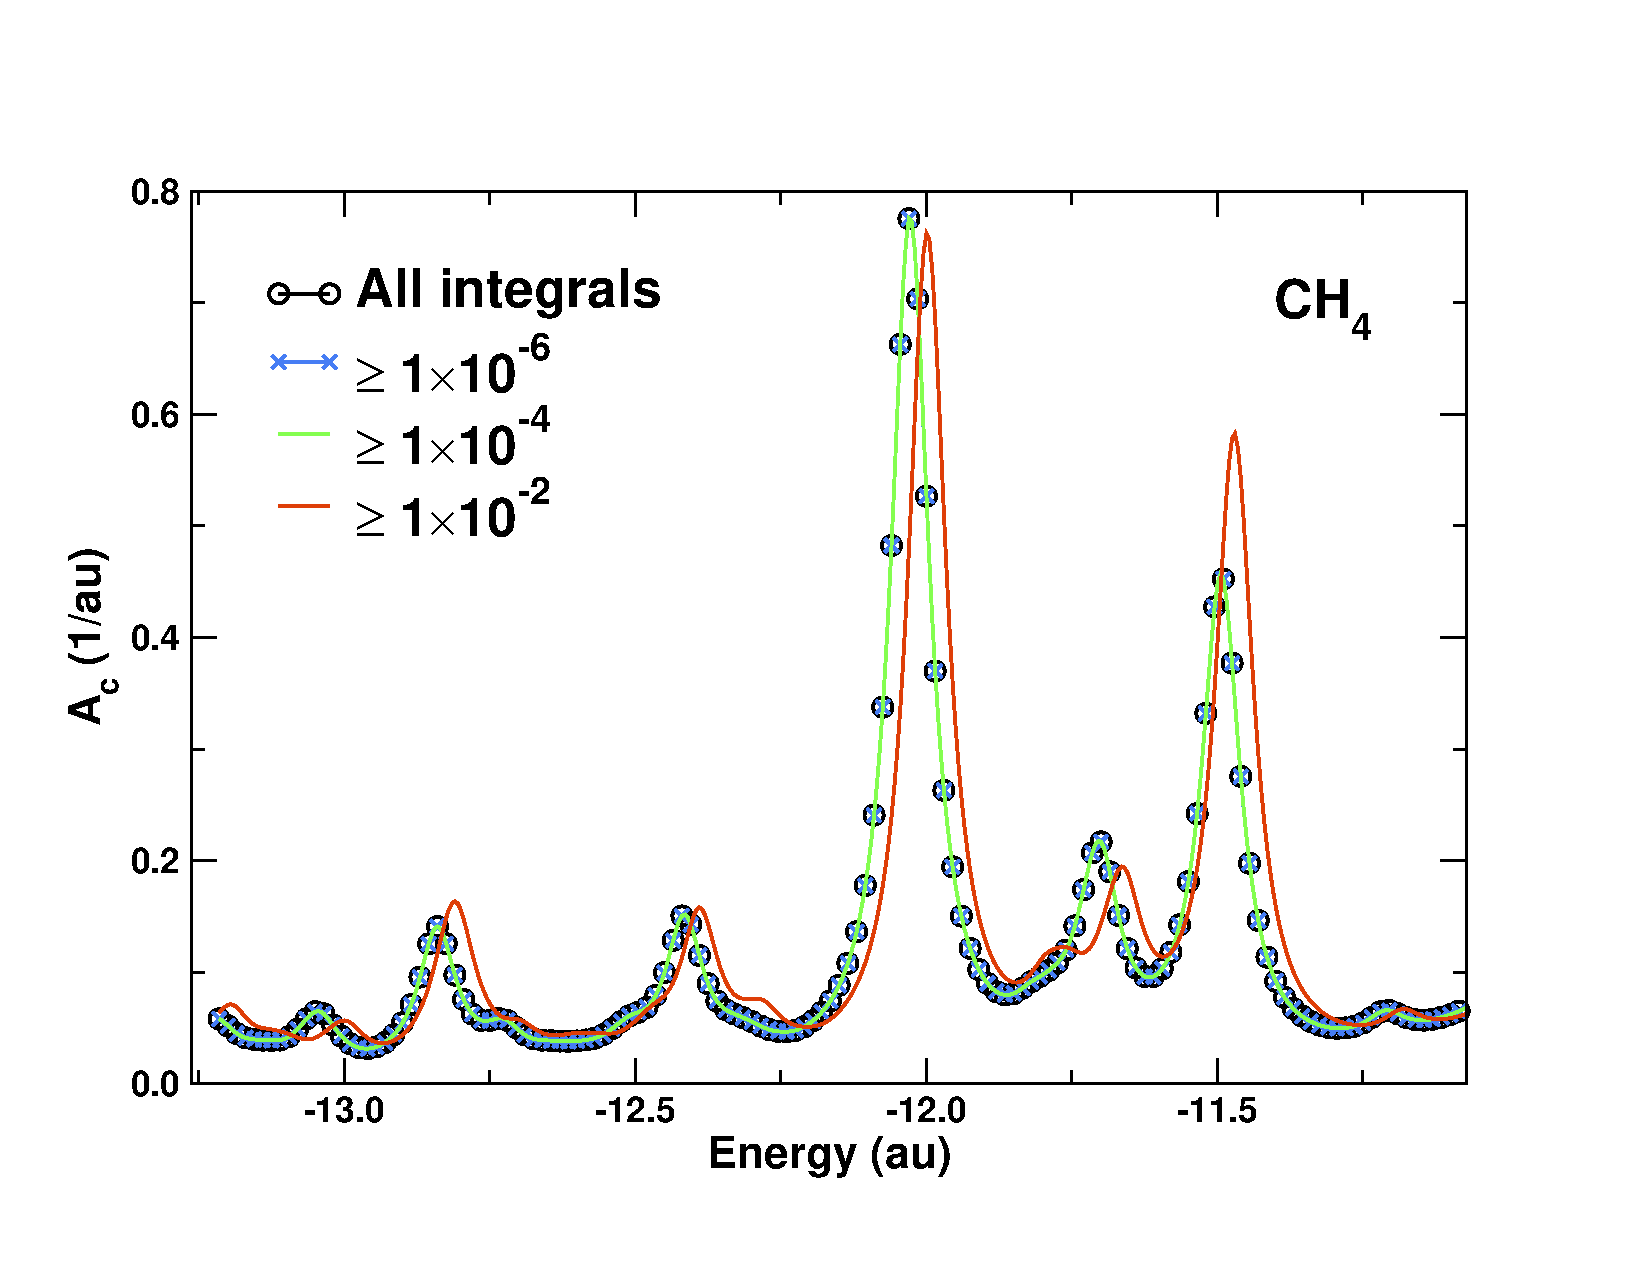
\includegraphics[scale=0.5,clip,
trim=1.1cm 1.2cm 3.0cm 1.8cm]{Fig03-SI.pdf}
\caption{\label{fig:cutoff}
Comparison of the satellite region of the core spectral function of CH$_4$ computed with the cc-pVDZ basis set and the full EOM-CCS method, as a function of potential integral cutoff.
}
\end{figure}
As discussed in the main manuscript, in order to reduce the storage requirements and computational demands of the EOM-CC method, we screen those $v_{pq}^{rs}$ integrals below a certain threshold after the SCF is fully converged. Figure \ref{fig:cutoff} shows a comparison between the spectral function of a typical system (CH$_4$) for different values of the cutoff parameter. We find that for the cutoff used in this paper (1$\times$10$^{-4}$ au) the EOM-CC results are indistinguishable from those obtained with all the integrals. With this cutoff, however, the performance of the method is increase by a factor of 10. This cutoff is also used in the DSE2 calculations, where it also has little effect in the accuracy, but produced only a modest improvement in performance. It should be noted that this integral trimming is not used in the GFCCSD and GFCC-i(2,3) calculations.

\subsection{Quasiparticle properties with the DZVP and cc-pVDZ basis sets}

Tables \ref{tbl:ebbas1} and \ref{tbl:ebbas2} summarize the core binding energies
for the different systems and methods calculated with the DZVP and cc-pVDZ basis
sets, respectively. While the KT, DSE2, and EOM-CC results show little
dependence on the basis set, for the GFCC methods the augmented Dunning basis
set seems not able to improve the results. To reduce the discrepancy of the GFCC
results, the employment of bare Dunning basis sets seems slightly better. For
the GFCCSD results, employing the aug-cc-pVDZ basis gives the MAE of 4.24 eV, in
comparison to the MAE of 3.57 eV brought by employing the bare cc-pVDZ basis.
Furthermore, the triple-$\zeta$ cc-pVTZ basis can systematically reduce the
discrepancies to even below 1 eV ($\sim$0.74 eV), which agrees with basis set
discussion in the previous EOM-CC and GFCC results for the core ionizations of
small molecules.\cite{mukherjee13_2625, sonia16_149901, peng18_4335}

\begin{table*}[t]
\caption{Comparison of the experimental core binding energies (in eV) to those obtained with the DZVP basis set, using the L and NL approximations to the cumulant and the 1-3 approximations of the EOM-CCS method, and their mean absolute errors (MAE).
}
\label{tbl:ebbas1}
\begin{ruledtabular}
\begin{tabular}{lddddddddddl}
\tbhr{System} & \tbhc{KT} &\tbhc{DSE2}& \tbhc{1$_{L}$} & \tbhc{2$_{L}$} & \tbhc{3$_{L}$} && \tbhc{1$_{NL}$} & \tbhc{2$_{NL}$} & \tbhc{3$_{NL}$} & \tbhc{Expt}& \tbhc{Ref} \\
\hline
CH$_4$&304.744&291.881& 286.990& 287.425& 286.994&& 290.412& 290.679& 290.415& 290.703&[\onlinecite{ch4spf}]\\
NH$_3$&422.523&405.466& 400.603& 400.815& 400.198&& 405.057& 405.177& 404.816& 405.520&[\onlinecite{nh3spf}]\\
H$_2$O&559.003&538.597& 534.795& 534.390& 533.705&& 539.498& 539.248& 538.843& 539.700&[\onlinecite{h2ospf}]\\
HF    &714.753&692.127& 689.876& 688.904& 688.313&& 694.174& 693.549& 693.178& 694.200&[\onlinecite{hfspf}] \\
Ne    &890.987&868.010& 867.661& 866.444& 866.109&& 870.935& 870.076& 869.842& 870.200&[\onlinecite{nespf}] \\
\hline
MAE   & 18.34 &1.32&   4.08 &   4.47 &   5.00 &&   0.34 &	0.32 &	 0.65 &        &		     \\
\end{tabular}
\end{ruledtabular}
\end{table*}
\begin{table*}[t]
\caption{Comparison of the experimental core binding energies (in eV) to those obtained with the cc-pVDZ basis set, using the L and NL approximations to the cumulant and the L$_c$, Q and F approximations of the EOM-CCS method, and their mean absolute errors (MAE). The KT results are obtained with Koopmans' Theorem.
}
\label{tbl:ebbas2}
\begin{ruledtabular}
\begin{tabular}{ldddddddddddl}
\tbhr{System} & \tbhc{KT} & \tbhc{DSE2}&\tbhc{\tiny{GFCCSD}} &\tbhc{\tiny{GFCC-i(2,3)}}  & \tbhc{1$_{NL}$} & \tbhc{2$_{L}$} & \tbhc{3$_{L}$} & \tbhc{1$_{L}$} & \tbhc{2$_{NL}$} & \tbhc{3$_{NL}$} & \tbhc{Expt}& \tbhc{Ref} \\
\hline
CH$_4$&305.17&292.56& 292.80 & 293.45 &286.98&287.84&287.44&290.54&291.08&290.83& 290.703&[\onlinecite{ch4spf}]\\
NH$_3$&422.78&406.26& 407.68 & 408.61 &400.67&401.35&400.81&405.13&405.55&405.23& 405.520&[\onlinecite{nh3spf}]\\
H$_2$O&559.25&539.30& 542.21 & 543.41 &534.53&534.74&534.15&539.32&539.46&539.10& 539.700&[\onlinecite{h2ospf}]\\
HF    &715.09&692.64& 696.78 & 698.19 &689.27&688.97&688.45&693.78&693.59&693.27& 694.200&[\onlinecite{hfspf}] \\
Ne    &891.59&868.17& 874.52 & 874.52 &866.50&865.87&865.57&870.16&869.73&869.52& 870.200&[\onlinecite{nespf}] \\
\hline
MAE   & 18.71 &1.32& 2.73& 3.57 &  4.48 &  4.31 &  4.78 &  0.28 &  0.35 &  0.53 &	 &		       \\
\end{tabular}
\end{ruledtabular}
\end{table*}

Tables \ref{tbl:zbas1} and \ref{tbl:zbas2} summarize the core quasiparticle strengths for the different systems and methods calculated with the DZVP and cc-pVDZ basis sets, respectively.
\begin{table*}[t]
\caption{Comparison of the quasiparticle strengths obtained with the DZVP basis set, using the L and NL approximations to the cumulant and the 1-3 approximations of the EOM-CCS method.
}
\label{tbl:zbas1}
\begin{ruledtabular}
\begin{tabular}{lddddddddddl}
\tbhr{System} & & \tbhc{DSE2} & \tbhc{1$_{L}$} & \tbhc{2$_{L}$} & \tbhc{3$_{L}$} && \tbhc{1$_{NL}$} & \tbhc{2$_{NL}$} & \tbhc{3$_{NL}$} &&\\
\hline
CH$_4$&&0.79&  0.60&  0.61&  0.59&&  0.70&  0.71&  0.69&&\\
NH$_3$&&0.77&  0.60&  0.61&  0.58&&  0.71&  0.71&  0.69&&\\
H$_2$O&&0.75&  0.63&  0.62&  0.59&&  0.73&  0.72&  0.70&&\\
HF    &&0.76&  0.68&  0.66&  0.64&&  0.76&  0.74&  0.72&&\\
Ne    &&0.78&  0.76&  0.73&  0.72&&  0.80&  0.78&  0.77&&\\
\end{tabular}
\end{ruledtabular}
\end{table*}
\begin{table*}[t]
\caption{Comparison of the quasiparticle strengths obtained with the cc-pVDZ basis set, using the L and NL approximations to the cumulant and the 1-3 approximations of the EOM-CCS method.
}
\label{tbl:zbas2}
\begin{ruledtabular}
\begin{tabular}{ldddddddddddd}
\tbhr{System} & \tbhc{DSE2}&\tbhc{GFCCSD} &\tbhc{GFCC-i(2,3)}  & \tbhc{1$_{L}$} & \tbhc{2$_{L}$} & \tbhc{3$_{L}$} && \tbhc{1$_{NL}$} & \tbhc{2$_{NL}$} & \tbhc{3$_{NL}$} &\\

\hline
CH$_4$&0.80& 0.77& 0.81& 0.60&  0.63&  0.61&&  0.70&  0.72&  0.71&&\\
NH$_3$&0.78& 0.76& 0.81& 0.61&  0.63&  0.61&&  0.71&  0.73&  0.71&&\\
H$_2$O&0.78& 0.71& 0.82& 0.64&  0.65&  0.63&&  0.74&  0.74&  0.72&&\\
HF    &0.79& 0.79& 0.84& 0.70&  0.69&  0.67&&  0.77&  0.76&  0.75&&\\
Ne    &0.81& 1.00& 1.00& 0.77&  0.76&  0.75&&  0.82&  0.81&  0.80&&\\
\end{tabular}
\end{ruledtabular}
\end{table*}
\begin{table}[t]
\caption{Scissors corrections used in Fig. \ref{fig:ac_sci}.}
\label{tbl:scicorr}
\begin{ruledtabular}
\begin{tabular}{lddddddl}
\tbhr{System} & &  & \tbhc{1$_{NL}$} & \tbhc{2$_{NL}$} & & &\\
\hline
CH$_4$&&&     1.9 &1.1 &  &  &\\
NH$_3$&&&     6.2 &1.6 &  &  &\\
H$_2$O&&&     8.8 &1.8 &  &  &\\
HF    &&&    10.4 &2.1 &  &  &\\
Ne    &&&    10.2 &1.5 &  &  &\\
\end{tabular}
\end{ruledtabular}
\end{table}

\subsection{Full comparison of the spectral function as a function of basis set, level of CCS approximation and cumulant form}

Figures \ref{fig:acbas1} and \ref{fig:acbas2} shows a comparison of the core spectral function of the $10e$ systems computed with the DZVP and cc-pVDZ basis sets, respectively, and the 3$_{NL}$ approach, as a function of EOM-CCS approximation.
\begin{figure}[t]
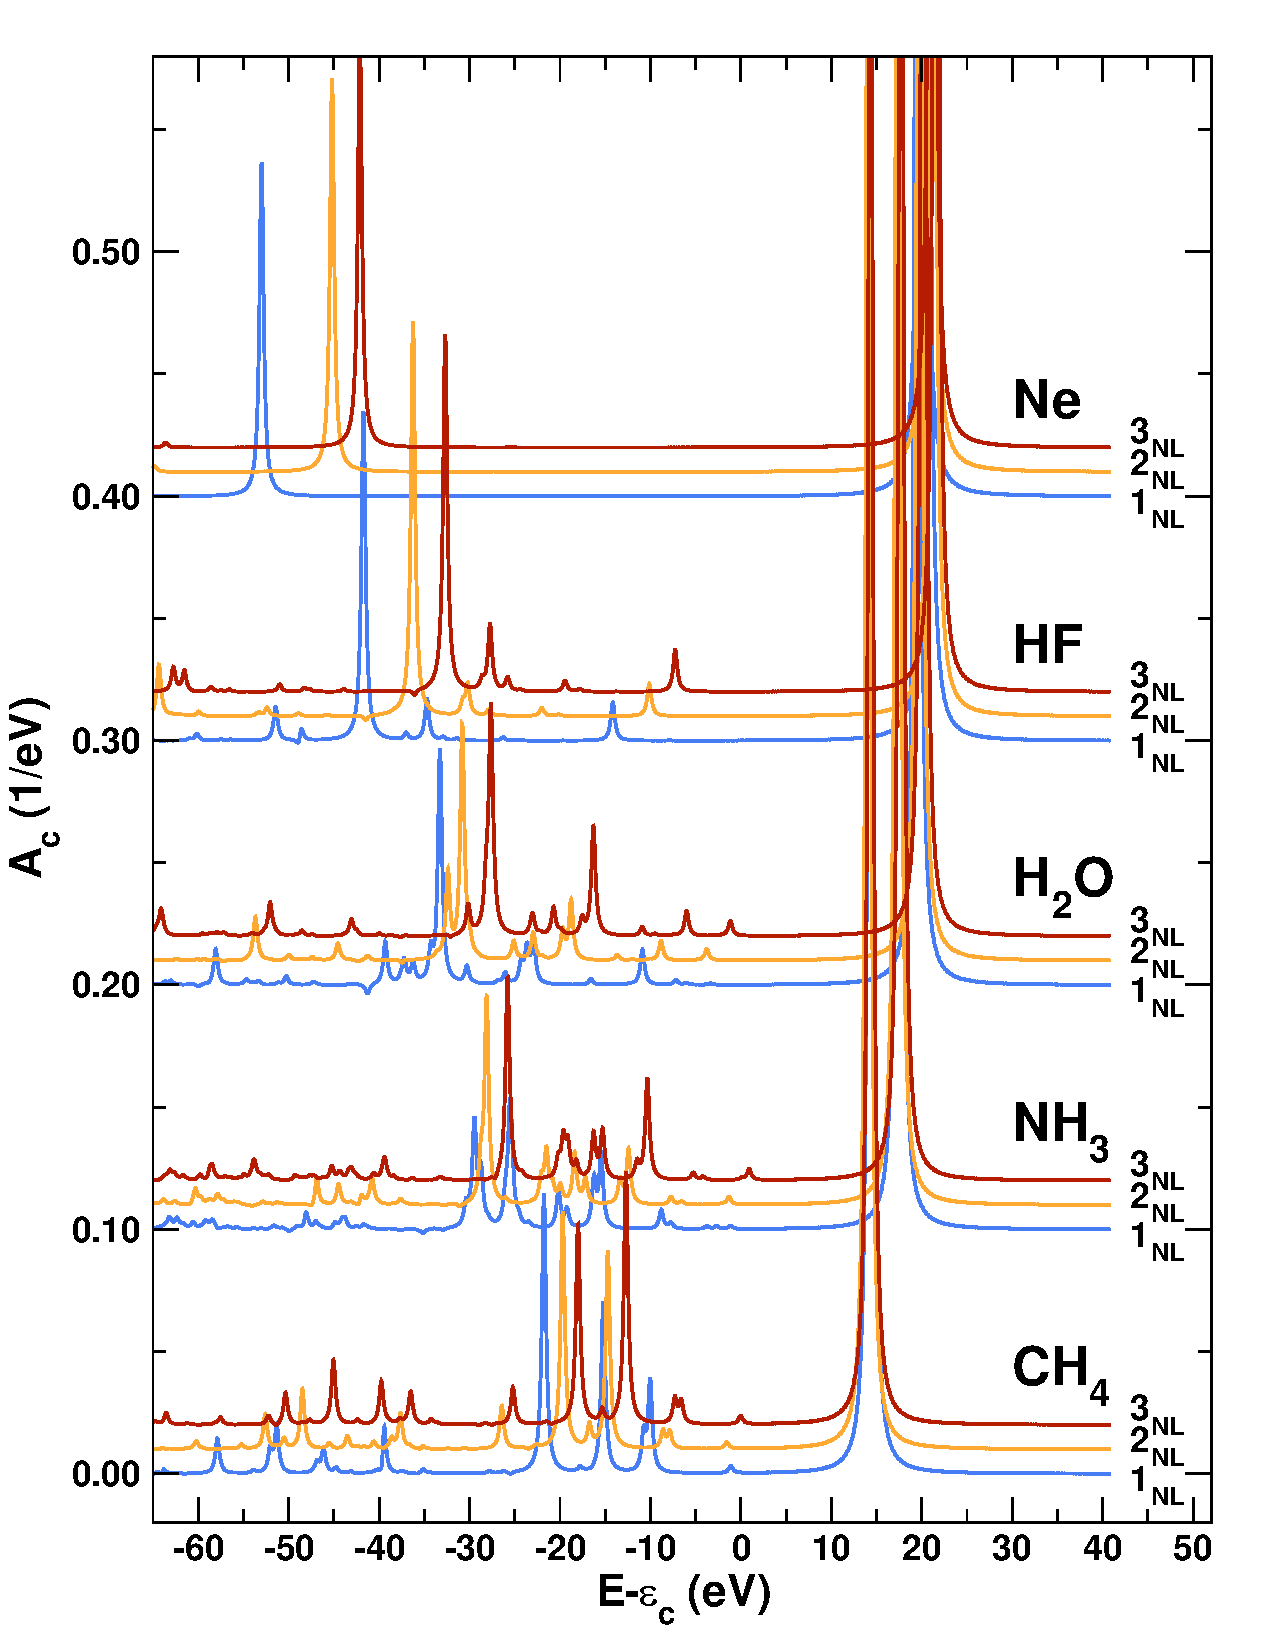
\includegraphics[scale=0.40,clip]{Fig04-SI.pdf}
\caption{\label{fig:acbas1}
Core spectral function $A_c$ of the $10e$ systems computed with the DZVP basis set, as a function of EOM-CCS approximation 1$_{NL}$ (blue), 2$_{NL}$ (orange), and 3$_{NL}$ (red).
}
\end{figure}
\begin{figure}[t]
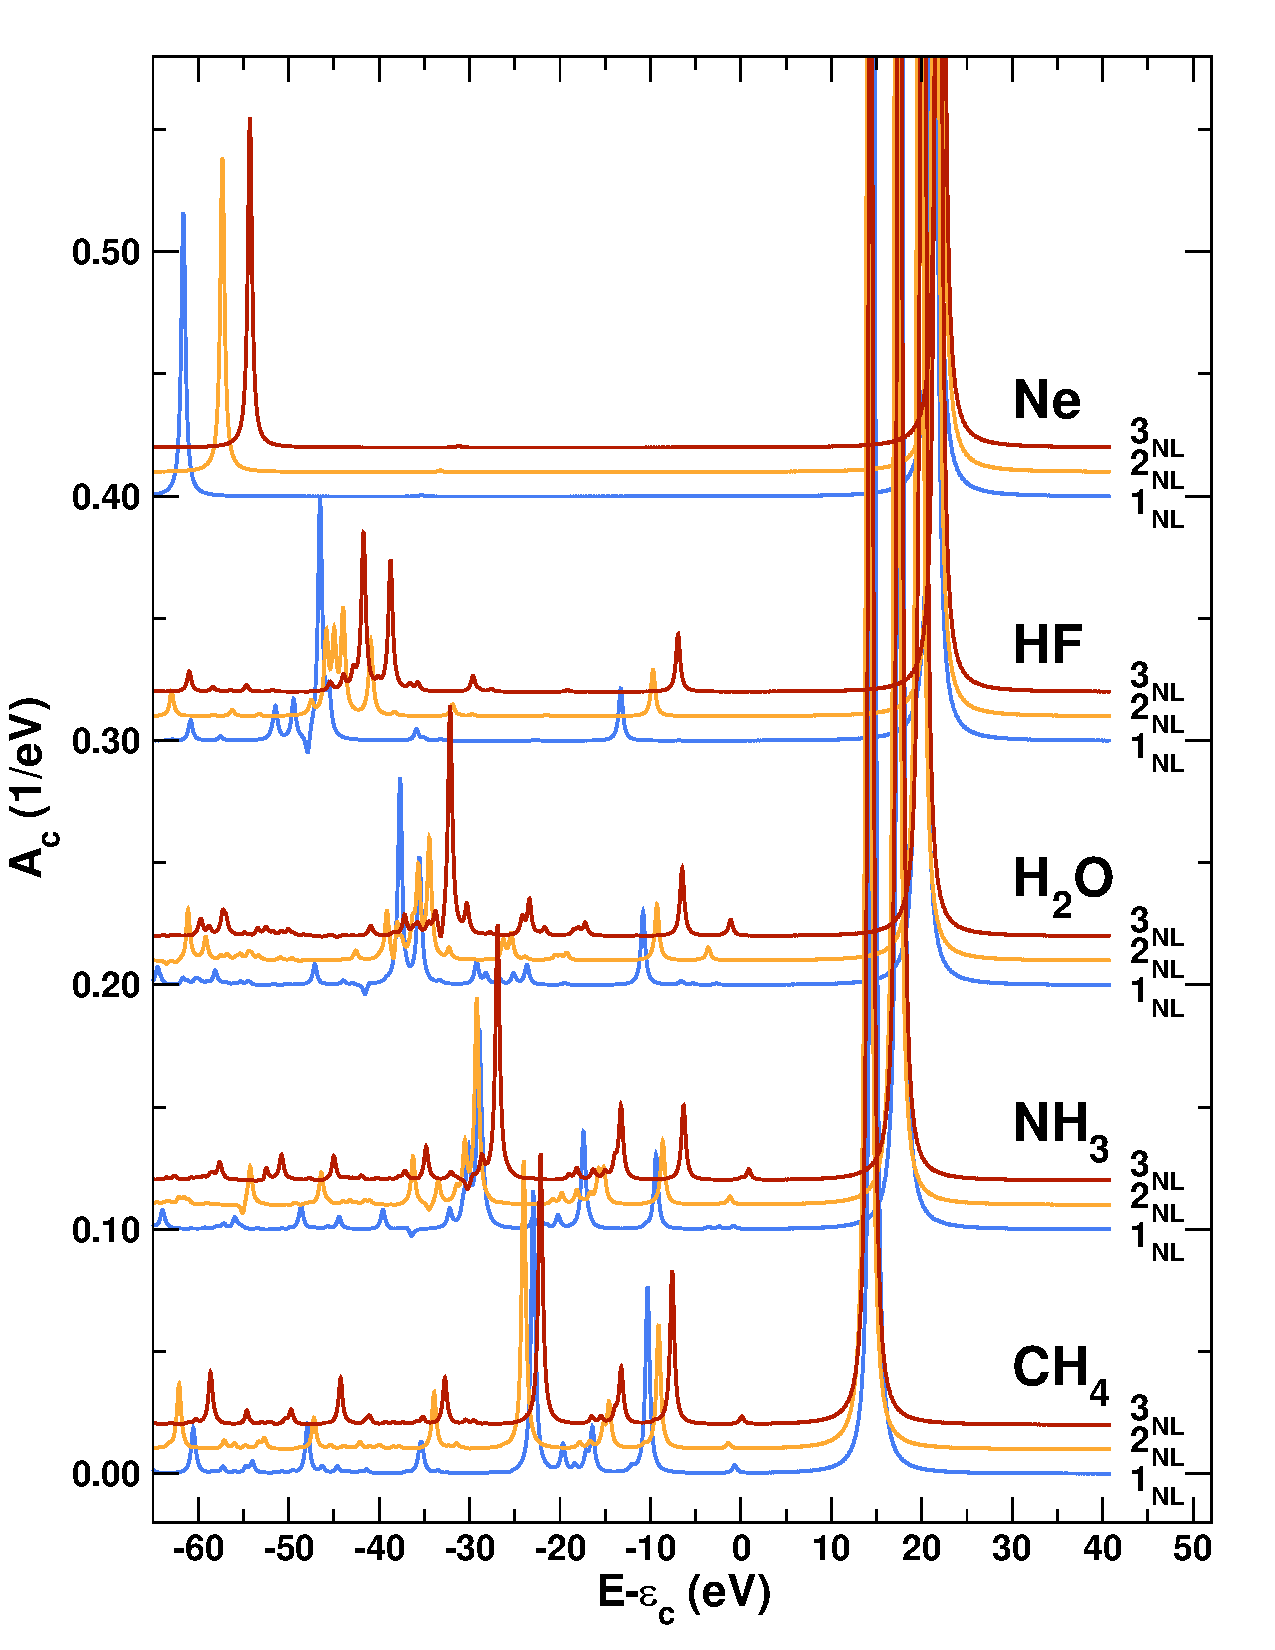
\includegraphics[scale=0.40,clip]{Fig05-SI.pdf}
\caption{\label{fig:acbas2}
Core spectral function $A_c$ of the $10e$ systems computed with the cc-pVDZ basis set, as a function of EOM-CCS approximation 1$_{NL}$ (blue), 2$_{NL}$ (orange), and 3$_{NL}$ (red).
}
\end{figure}

\subsection{Effect of the CCS approach on the gap between the quasiparticle and the satellites}

Figure \ref{fig:ac_sci} shows a comparison of the spectral functions with a scissors correction applied to the 1$_{NL}$ and 2$_{NL}$ approaches in such a way that the satellite regions become aligned with those in the 3$_{NL}$ approach. After the correction is applied, the 2$_{NL}$ approximation is shown to give results that are almost identical to the full approach. Despite showing some noticeable differences, 1$_{NL}$ approximation shows reasonable agreement in the overall distribution of the satellite intensity. The scissors corrections for each system and method are shown in Table \ref{tbl:scicorr}. Interestingly, while the corrections required for the 1$_{NL}$ approximation are clearly system-dependent, in the case of the 2$_{NL}$ approximation the corrections are almost constant, suggesting that an overall scissors correction can be used to simulate the results of the more expensive full approach.

\begin{figure}[t]
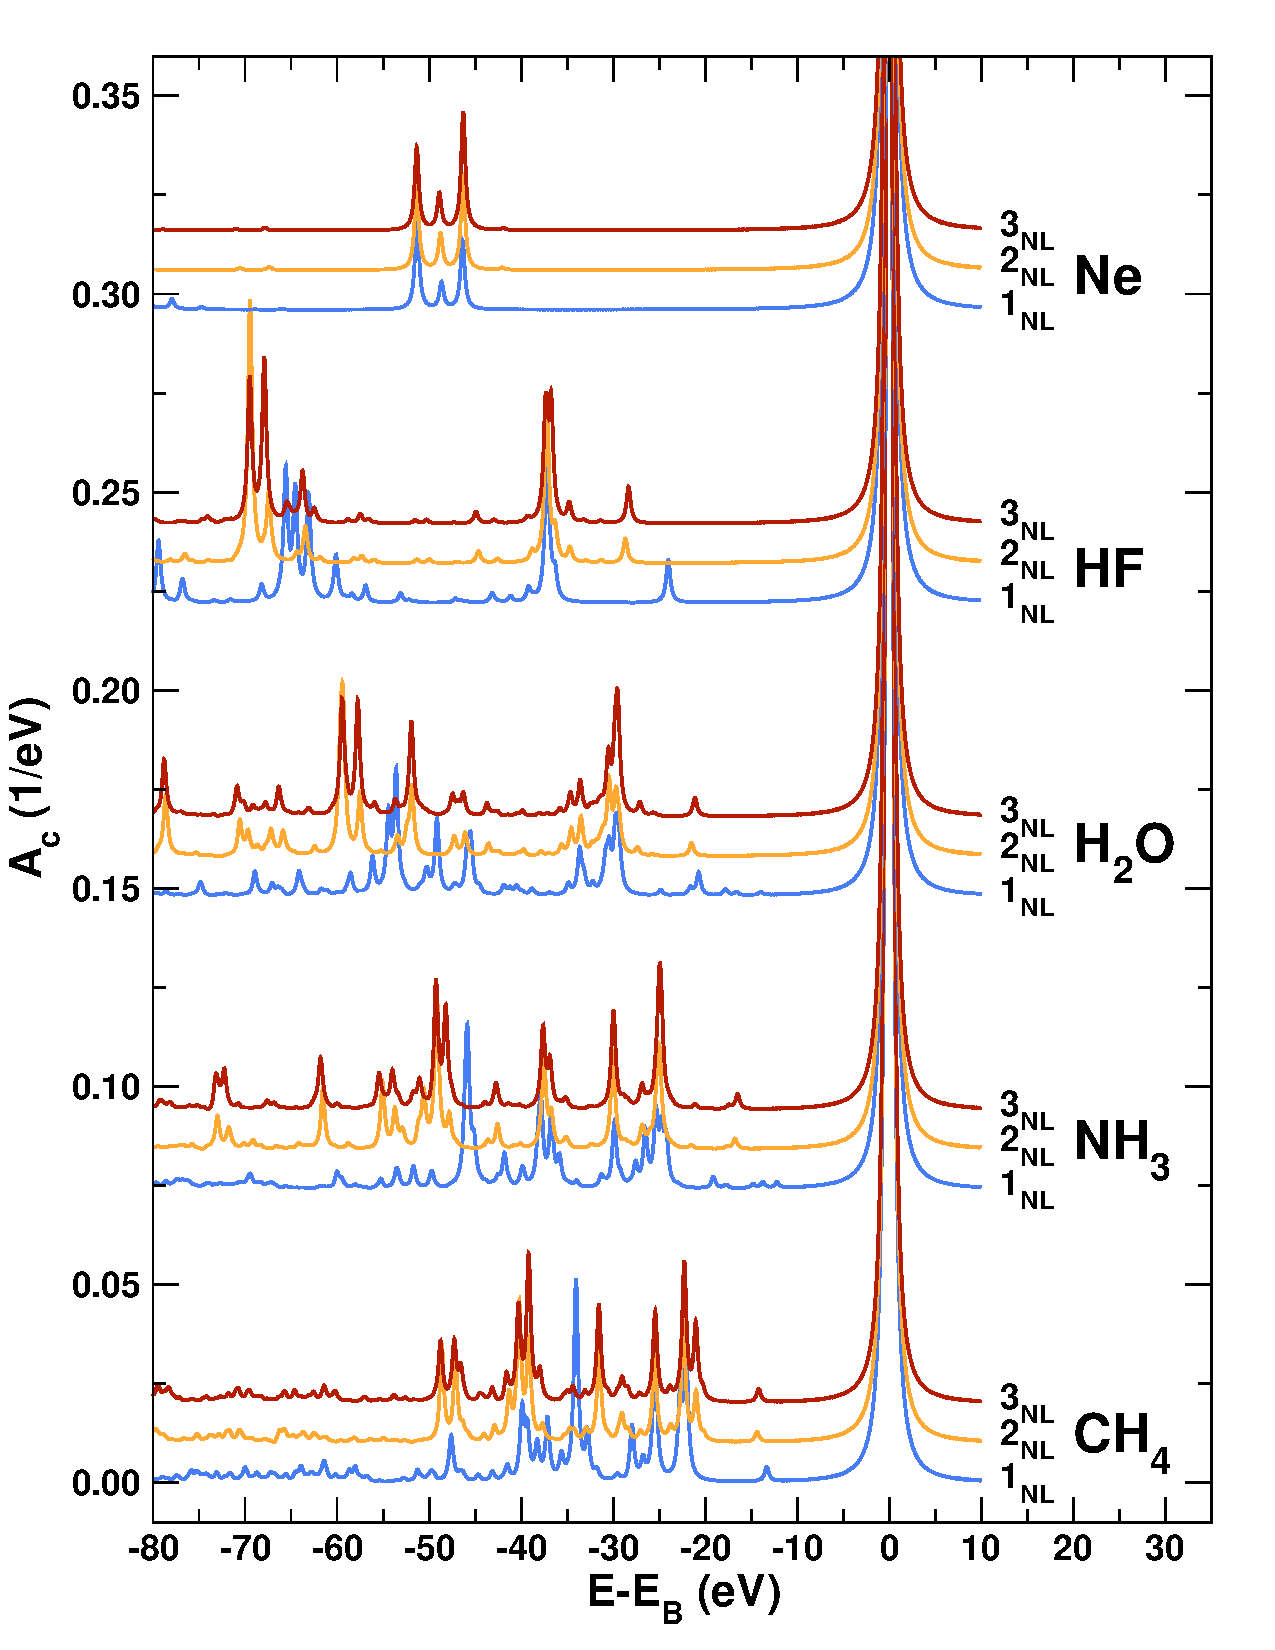
\includegraphics[scale=0.40,clip]{Fig06-SI.pdf}
\caption{\label{fig:ac_sci}
Comparison of the spectral functions with a scissors correction (see Table \ref{tbl:scicorr}) applied to the 1$_{NL}$ (blue) and 2$_{NL}$ (orange) approximations in such a way that the satellite regions become aligned with those of 3$_{NL}$ (red).
}
\end{figure}

\bibliography{EOM-CC-Cumulant-Approach}
\bibliographystyle{apsrev}

\end{document}

